\documentclass[11pt, oneside]{amsart}
\usepackage{geometry}
\geometry{letterpaper}
\usepackage{graphicx}
\usepackage{amssymb}
\usepackage{microtype}
\usepackage[dvipsnames]{xcolor}
\usepackage{tikz}
\usepackage{todonotes}
\usepackage{listings}
\usepackage{tabularx}
\usepackage{booktabs}
\usepackage{hyperref}

\lstset{frame=single,
	language=c++,
	basicstyle=\small\ttfamily,
	breaklines=false,
	tabsize=4,
	commentstyle=\color{OliveGreen},
	keywordstyle=\bfseries\color{NavyBlue},
	emph={
	    vec2, vec3, u8vec3, u16vec2, u16vec3, mat4, quat, integer, real, string, AnyID, Color, Scalar, list, optional, variant, null,
	},emphstyle={\bfseries}}

\colorlet{punct}{red!60!black}
%\definecolor{background}{HTML}{EEEEEE}
\definecolor{delim}{RGB}{20,105,176}
\colorlet{numb}{magenta!60!black}

\definecolor{codeindent}{HTML}{CCCCCC}
\newcommand{\indentrule}{\color{codeindent}\vrule\hspace{2pt}}

\lstdefinelanguage{json}{
    basicstyle=\small\ttfamily,
    numbers=left,
    numberstyle=\scriptsize,
    stepnumber=1,
   	tabsize=4,
    numbersep=8pt,
    showstringspaces=false,
    breaklines=true,
    %backgroundcolor=\color{background},
    literate=
     *{0}{{{\color{numb}0}}}{1}
      {1}{{{\color{numb}1}}}{1}
      {2}{{{\color{numb}2}}}{1}
      {3}{{{\color{numb}3}}}{1}
      {4}{{{\color{numb}4}}}{1}
      {5}{{{\color{numb}5}}}{1}
      {6}{{{\color{numb}6}}}{1}
      {7}{{{\color{numb}7}}}{1}
      {8}{{{\color{numb}8}}}{1}
      {9}{{{\color{numb}9}}}{1}
      {:}{{{\color{punct}{:}}}}{1}
      {,}{{{\color{punct}{,}}}}{1}
      {\{}{{{\color{delim}{\{}}}}{1}
      {\}}{{{\color{delim}{\}}}}}{1}
      {[}{{{\color{delim}{[}}}}{1}
      {]}{{{\color{delim}{]}}}}{1},
}

\lstdefinelanguage{flatbuffers}[]{c++}{
	keywords={table, struct,  include, root_type, union, uint64, uint32, int64, double, string, required, float, namespace},
	comment=[l]{//},
	basicstyle=\footnotesize\ttfamily,
	numbers=left,
	numberstyle=\scriptsize,
	stepnumber=1,
	numbersep=8pt,
	showstringspaces=false,
	breaklines=true,
}

\usetikzlibrary{shapes,arrows}

\tikzstyle{block} = [rectangle, draw, fill=blue!20,
    text width=5em, text centered, rounded corners, minimum height=4em, node distance=3cm]
\tikzstyle{line} = [draw]


\title{NOODLES v0.2: A Protocol Specification}
\author{Nicholas Brunhart-Lupo}

\begin{document}
\maketitle
\tableofcontents

\section{Introduction}

This document entails a specification for a distributed scene-graph wireline protocol suitable as a substrate for shared interactive visualizations. It also lays out concepts for the supporting implementations that would provide such visualizations.


\section{Rationale \& Design Goals}

\begin{itemize}
\item The intent of this document is simplicity, to get a working version implemented so that further improvements can be identified.
\item The structure here is not intended to mirror the use-case of the HTML DOM + Javascript where code is shipped to clients. That would be restrictive, as it requires the clients either interpret or compile and run code on command. Some clients, such as integrated head mounted systems, do not allow compilation, or are not sufficient computing platforms.
\item Trying to mirror just the HTML DOM part has issues as well; a number of 3D declarative implementations (like QML 3D), all operate on a scenegraph under the hood. It seems more fruitful to just target the scenegraph for modification, and perhaps (as part of the server library) have a declarative component there.
\item A shared document is desired here, as opposed to the standard browser case where every client has their own copy of state.
\item Code listings are provided as an example and for exposition only. Clients and servers may be written in any language as long as they conform to the proper wireline protocol.
\end{itemize}


\section{Architecture}

The system envisions the use of four components, two of which fall under this specification.

\begin{figure}[htbp]
\begin{center}

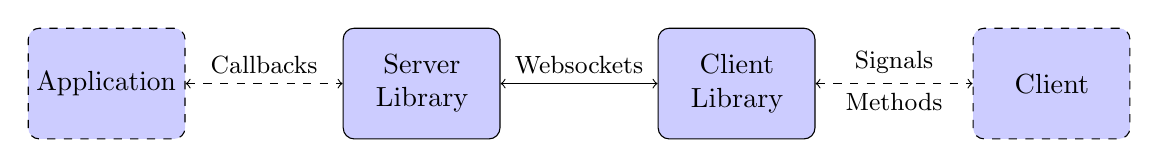
\begin{tikzpicture}[node distance = 4cm, auto]
    % Place nodes
    \node [block, dashed] at (0,0) (server) {Application};
    \node [block] at (4,0) (serverlib) {Server Library};
    \node [block] at (8,0) (clientlib) {Client Library};
    \node [block, dashed] at (12,0) (client) {Client};
    % Draw edges
    \path [line, dashed,<->] (server) -- node[above] {\small Callbacks} (serverlib);
    \path [line, <->] (serverlib) -- node[above] {\small Websockets}  (clientlib);
    \path [line, dashed, <->] (clientlib) -- node[above] {\small Signals} node[below] {\small Methods} (client);
\end{tikzpicture}

\caption{System architecture. Note that there may be more than one client. Elements with solid lines fall under this specification.}
\end{center}
\end{figure}

The Server Library presents a visualization to one or more connected clients through a synchronized scenegraph. Client requests and messages are passed on for handling to the application code, which can manipulate the scenegraph in response. These changes are then published and sent to clients.

The Client Library connects to a server, and maintains the synchronized scenegraph. This scenegraph is query-able by the client. Clients then can interpret and present the scenegraph to the user in the way they see fit. For example, an immersive graphics engine client can draw the scenegraph as is, while a 2D client can choose to present only a subset of the graph. A command line (i.e. Python) client may ignore the scenegraph completely to merely make use of the messaging and method invocation functionality. This also allows each client to customize the interactions available in a way that best aligns with their form factor.

\subsection{Communication}

Communication between the libraries is achieved over Websocket connections. All messages are sent over the binary channel of the WebSocket using Flatbuffers.

Client-to-client notification is not supported, and must first pass through the server.

The bulk of communication is from server to client.

This spec is intended to be implemented in a secure network, with the presumption that those that connect to the server are trusted. Provision for security will come later, as is the case with everything, because security is hard and makes my brain bleed.

\subsubsection{Flatbuffers}

For performance reasons, the \textit{in-situ} capabilities of the serialization medium down-selected available options to Flatbuffers and Cap'n'proto. Both were explored. Table~\ref{tab:serial_comp} compares the two in rough terms. In the end Flatbuffers won out due to more language support out of the box.

\begin{table}[htbp]
\begin{tabularx}{.99\textwidth}{p{.9in}XX}
	\toprule
	~ & \textbf{Pro} & \textbf{Con} \\
	\midrule
	\textbf{Cap'n'Proto} & Created by Protobuf developers, strong pedigree. Excellent JSON inter-operation.  & More complex internal formats. Fewer languages supported out of the box. Some packages for other languages are of lower quality. Default serialization code has performance issues.\footnote{It requires a memory clear on any buffer before use.} \\
	\midrule
	\textbf{Flatbuffers} & More languages supported out of the box. Simple internal format, more format features (such as maps, field deprecation, evolution). Easier to obtain performance increases using existing serialization code. & API for some languages is horrible. Some languages require schema to have specific design, adding indirection. \\
	\bottomrule
\end{tabularx}
	\caption{Serialization Format Comparison}
	\label{tab:serial_comp}
\end{table}

\section{Concepts}

\begin{figure}[htbp]
\begin{center}
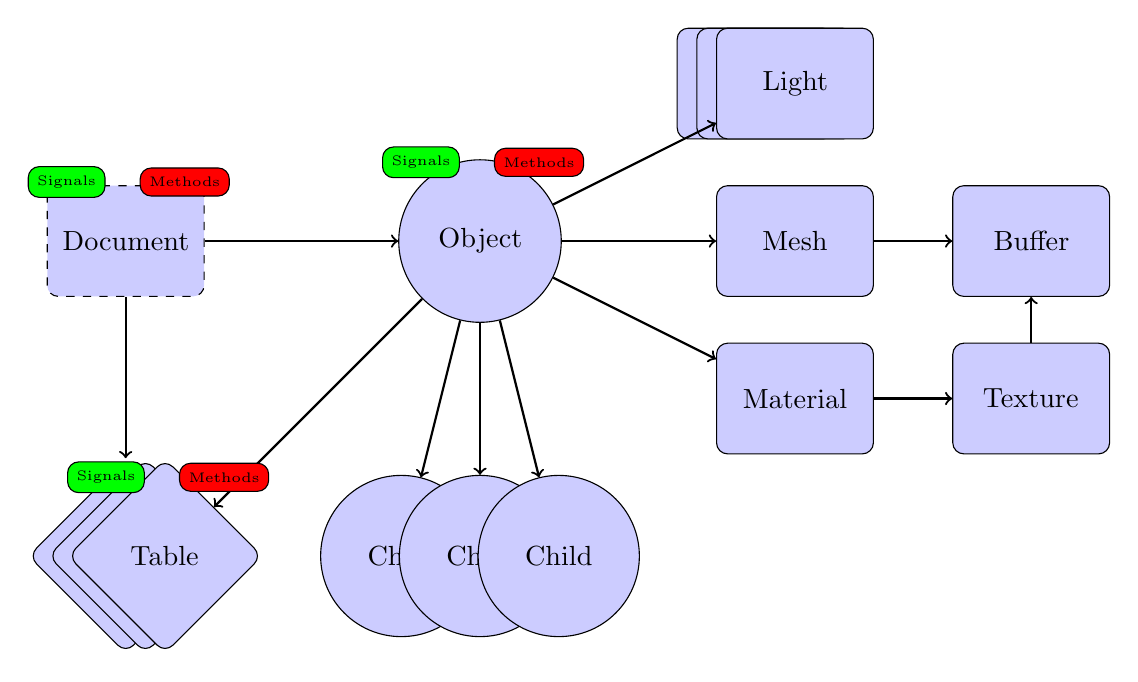
\begin{tikzpicture}
	% Place nodes
	\node [block, rectangle, dashed] at (.5,4) (doc) {Document};
	\node [draw, fill=red, rounded corners] at (1.25,4.75) {\tiny Methods};
	\node [draw, fill=green, rounded corners] at (-.25,4.75) {\tiny Signals};

	\node [block, circle] at (5,4) (root) {Object};
	\node [draw, fill=red, rounded corners] at (5.75,5) {\tiny Methods};
	\node [draw, fill=green, rounded corners] at (4.25,5) {\tiny Signals};

	\node [block] at (9,2) (material) {Material};
	\node [block] at (9,4) (mesh) {Mesh};
	\node [block] at (12,2) (texture) {Texture};
	\node [block] at (12,4) (buffer) {Buffer};

	\node [block] at (8.5,6) (light) {Light};
	\node [block] at (8.75,6) (light) {Light};
	\node [block] at (9,6) (light) {Light};

	\node [block, circle] at (4,0) (child0) {Child};
	\node [block, circle] at (5,0) (child1) {Child};
	\node [block, circle] at (6,0) (child2) {Child};

	\node [block, diamond] at (.5,0) (table1) {Table};
	\node [block, diamond] at (.75,0) (table2) {Table};
	\node [block, diamond] at (1,0) (table3) {Table};


	\draw[->, thick](doc)--(root);

	\draw[->, thick](root)--(table3);

	\draw[->, thick](root)--(child0);
	\draw[->, thick](root)--(child1);
	\draw[->, thick](root)--(child2);

	\draw[->, thick](root)--(mesh);
	\draw[->, thick](root)--(material);
	\draw[->, thick](root)--(light);

	\draw[->, thick](material)--(texture);

	\draw[->, thick](texture)--(buffer);
	\draw[->, thick](mesh)--(buffer);

	\draw[->, thick](doc)--(table1);

	\node [draw, fill=green, rounded corners] at (.25,1) {\tiny Signals};
	\node [draw, fill=red, rounded corners] at (1.75,1) {\tiny Methods};
\end{tikzpicture}

\caption{Document structure.}
\end{center}
\end{figure}



The objective of the system is to synchronize, as best as possible, the document between the client and the server. This is accomplished through the use of discrete messages.

\subsection{Document}

The Document represents the visualization. It is an entity-component model, with an Object as the core entity, and Tables being a secondary entity.

The document is implicit. The other elements are explicit.

\subsection{Identifiers}
Identifiers are a pair of 32-bit unsigned integers; the first being a slot number, and the second being a generation count. This allows non-hashed storage, as there should be no two elements with the same slot number, so it can be used as an index in an array. The generation number is used to help identify if a slot has been recycled by the server, and thus allow detection of stale identifier use.

An identifier where either the slot and generation are the maximum unsigned integer value is the `null' ID.

\subsection{Objects}
Each object is provided with an Object ID. Objects are rendered in a hierarchy, starting from a root object with the ID 0. Objects can have any number of children.

Each object is a possibly render-able object, and has a transformation, an optional name, a parent Object ID, a mesh (what to draw), a material (how to draw it), a number of lights, and links to tables. Objects also have a set of string tags, and attached methods and signals. Objects can also be instance rendered.

Objects are mutable.

\subsection{Tables}
Tables are a structured way to transmit row oriented data. They consist of a header (list of column names), and rows. Attached signals and methods are used to allow clients to modify the data in the table or fetch records (but only when first subscribed to).

\subsection{Signals and Methods}
Signals are notifications from the server to the client. They may contain data, and may come from the document, objects, or tables.

Methods are requests to the server from the client. They may take a set of data parameters, and they may return data as well. They must have a contextual object that they are called on, otherwise they are called on the Document. During the course of a method invocation, signals from the server could be generated.

Each method invocation is tracked by a client-generated arbitrary string. These shall be unique and never re-used. For servers, every method must generate a reply message; the only exception is if the client did not provide an invocation identifier string.

There is a possibility that a method could be called on an object, that is then subsequently deleted, or replaced. In this case, a reply is still generated, and not squashed by the server. Thus a client should be able to handle replies on objects that no longer exist.

Methods and signals are immutable.

\subsection{Buffers}
A buffer is an opaque block of bytes. This allows for efficient storage and transfer of large assets. These assets can be sent either inline through the WebSocket, or can be supplied through a URL that the client can fetch the buffer from.

Buffers are immutable and referenced from meshes and textures.

\subsection{Mesh}
Meshes define the geometry that is to be rendered. They consist of references to a buffer for number of components (see Table~\ref{tab:mesh_comp}).

Meshes are mutable.

\begin{table}
	\begin{tabular}{cccc}
		\toprule
		\textbf{Component} & \textbf{Type} & \textbf{Value Type} & \textbf{Count} \\
		\midrule
		Position & Vertex & float & 3 \\
		Normals & Vertex & float & 3 \\
		TexCoords & Vertex & unsigned short & 2 \\
		Colors & Vertex & unsigned byte & 4 \\
		Lines & Index & unsigned short & 2 \\
		Triangles & Index & unsigned short & 3 \\
		\bottomrule
	\end{tabular}
	\caption{Mesh components}
	\label{tab:mesh_comp}
\end{table}

\subsection{Materials}
This should be a PBR based material, featuring basic elements: base color, metallic, roughness, including an optional texture for base colors. The material only applies to the node it is attached to. Note that though the material is specified in PBR, the client may use Phong or other interpretations of the specified material in order to meet performance goals. The material may also specify that blending should be used; the blending function is $src_{\alpha}$ and $1-src_{\alpha}$.

Materials are mutable.

\subsection{Textures}
Textures reference images (in Buffers) to be used by a material. Textures are mutable.

\subsection{Lights}
Lights describe illumination sources. They are mutable.

\section{Common Message Elements}
This section discusses common elements to both the server and client message portions of the specification.

\subsection{Any Type}
The any type is the foundation value type. it is composed as follows:

\lstinputlisting[language=flatbuffers, firstline=53, lastline=93, caption=Any Definition, label=listing:any]{"../interface/noodles.fbs"}

It is a discriminated union of text, integers, real, or bytes. It also contains a generic list, and string-keyed map. For efficiency, there is also a real-list and integer-list type which allow contiguous storage or access of those elements.

In method and signal API terms, real-lists and integer-lists are coerce-able. That means, for example, that a list of reals may be provided by the \texttt{RealList} type, or as a \texttt{AnyList} of \texttt{Real}.

\section{Server Messages}
\label{sec:server_message}

Here we discuss the messages that are sent from the server to the client.

Almost all components have strict lifetimes defined by creation and deletion messages. Some messages are also used to update an existing component. Therefore, if a create-update message is received by the client for a component/entity of an ID that it has never seen before, that is the creation milestone. Otherwise, it is an update message. Update messages are treated differently; presence of a key in the update message table implies that the new value should overwrite a previously received value for that key.

\subsection{Root Message}

The server sends messages by the root type \texttt{ServerMessages}. This is an array of a union of creation/deletion messages.

\lstinputlisting[language=flatbuffers, firstline=198, lastline=232, caption=Server Root Messages]{"../interface/noodles_server.fbs"}

\subsection{Objects}

Objects are created, updated and destroyed in Listing~\ref{listing:obj}.

\lstinputlisting[language=flatbuffers, firstline=42, lastline=68, caption=Object Messages, label=listing:obj]{"../interface/noodles_server.fbs"}

Each element is optional, with the exception of the object id.

If the object ID has not been seen before by the client, it is assumed to be a new object. If there is no transform in the message, it is assumed to be the identity.

If the object ID has been seen before and not deleted, it should update the existing object with the elements that are provided in the message. For example, an message for Object ID 5 that contains a transform will only update object 5's transform, and not change other elements. In another example, to detach a material from an object, an update message with a null material ID is used.

Instances of the underlying meshes are specified by a list of matrices, with a matrix per instance. Using column major ordering, Matrix~\ref{eqn.instances}, shows how position $p$, rotation $r$ (as a quaternion), color $c$, and scale $s$ are specified. Access is assumed to be by column, i.e.\ $M_0 = p$.

\begin{equation}
\label{eqn.instances}
\left(
\begin{array}{cccc}
p_x & c_r & r_x & s_x \\
p_y & c_g & r_y & s_y \\
p_z & c_b & r_z & s_z \\
0 & 0 & r_w & 0
\end{array}
\right)
\end{equation}

Text can be added to an object by means of the optional \texttt{TextDefinition} part of the message. Text is to be rendered how the client sees fit, with the orientation to be centered at the object, the text perpendicular to $+Z$ and up being $+Y$. The height of the text must be specified; the text will then automatically use the font information to compute the text width. If the optional width is specified, then the text shall, keeping the proper font aspect ratio, try to fill the bounds provided.

\subsection{Tables}

Tables are created and destroyed in the following messages.

\lstinputlisting[language=flatbuffers, firstline=155, lastline=165, caption=Table Messages, label=listing:tbl]{"../interface/noodles_server.fbs"}

Tables have names (which shall be unique), a metadata JSON string, methods, and signals.

\subsection{Buffers}

Buffers are created and destroyed in the following messages.

\lstinputlisting[language=flatbuffers, firstline=72, lastline=84, caption=Buffer Messages, label=listing:buff]{"../interface/noodles_server.fbs"}

Buffers are either inline (in the \texttt{bytes} field) or provided as a URL. If a URL is supplied the size of the buffer must be passed as well. If neither is supplied, the server has the data inline, but has deemed it too large to send immediately to avoid stalling clients. In this case, the server would do well to supply the data through another port and use the URL feature, but some servers are unable to do this. In this case, where both the bytes and URL feature are empty, the \texttt{url\_size} field must still be filled for client pre-allocation. At intervals, the client can send a refresh message to fill in the missing buffers to avoid burdening the websocket (see Section~\ref{sec:refresh_message} ).

\subsection{Geometry}

Geometries are created, and destroyed in the following messages.

\lstinputlisting[language=flatbuffers, firstline=127, lastline=150, caption=Geometry Messages, label=listing:geom]{"../interface/noodles_server.fbs"}

Limitations in Flatbuffer IDL require some notes here. Geometries are defined by ranges of a buffer for their components. These ranges, in the \texttt{ComponentRef} type, require a buffer, and also \textit{require} a start byte offset of the buffer, as well as a byte size field, and the byte stride between vertex elements.

The \texttt{min\_extent} and \texttt{max\_extent} fields are required so that clients can efficiently determine culling boundaries.

The position field is required. The other vertex components (\texttt{normals, texCoords, colors}) are optional, but recommended. If there is no normal, the mesh should be rendered without lighting to avoid graphical artifacts. If there are no texture coordinates, the coordinate $(0,0)$ should be assumed for each vertex. If there are no colors, the color $(1,1,1,1)$ should be assumed for each vertex.

Index elements are specified in \texttt{lines} and \texttt{triangles}. Only one of these should be active. These specify the indices for line segments and triangles respectively. The stride for these components must be zero, i.e. they must be tightly packed.

\subsection{Texture}

Textures are created, updated, and destroyed in the following messages.

\lstinputlisting[language=flatbuffers, firstline=103, lastline=110, caption=Texture Messages, label=listing:tex]{"../interface/noodles_server.fbs"}

Textures, specify a buffer range for an image. For portability, these are to be in the on-disk format for PNG, JPG, or EXR. KTX is also allowed, but the user should be aware that not all clients can support it.

\subsection{Material}

Materials are created, updated, and destroyed in the following messages.

\lstinputlisting[language=flatbuffers, firstline=88, lastline=99, caption=Material Messages, label=listing:mat]{"../interface/noodles_server.fbs"}

The \texttt{color} key defines colors in the range of $0 - 1$ for $r,g,b,a$. Other PBR parameters are also in the $0 - 1$ range. The texture ID field is optional, and could also be null to indicate no texture.

Materials can be updated and are not immutable.

\subsection{Lights}

 Lights are created, updated, and destroyed in the following messages.

 \lstinputlisting[language=flatbuffers, firstline=114, lastline=123, caption=Light Messages, label=listing:light]{"../interface/noodles_server.fbs"}

 The \texttt{color} key defines colors in the range of $0 - 1$ for $r,g,b$. Intensity of the light is unbounded.


\subsection{Signals \& Methods}

Signals and Methods are created, and destroyed in the following messages.

\lstinputlisting[language=flatbuffers, firstline=10, lastline=25, caption=Signals Messages, label=listing:sig_meth]{"../interface/noodles_server.fbs"}

Methods must be provided with a human friendly name. Two methods may not share the same name; there is no overloading. Documentation is recommended, but not required, as is return value documentation. Argument information must be provided, at the very least given a name. You may not call a method with more arguments then as specified; use an argument that takes an array type to permit this option.

Signal must be provided with a human friendly name, and also may not share the same name. Arguments follow the same requirements as methods.

\subsection{Signal Invoke \& Method Reply}

Signals may be invoked on the client and client methods replied to with the following messages.

\lstinputlisting[language=flatbuffers, firstline=180, lastline=194, caption=Communication, label=listing:sig_meth_iv]{"../interface/noodles_server.fbs"}

Either only \texttt{on\_object} or \texttt{on\_table} or neither must be set, to indicate context. Signals may NOT be invoked on a context that does not have them attached.

Method replies must have a previously given method invocation identifier (see Section \ref{sec:method_invoke} ). If the method could not be executed, an exception field is filled instead of data. The method should let the caller know what went wrong, and who should fix it. Consider three cases:

\begin{description}
	\item[Caller] The caller of the method (client) violated the contract of the method; incorrect number of arguments, bad argument content, etc.
	\item[Server/Application] A problem occurred with the application. The app itself encountered a problem; for example a client asking to load some data, but the server doesn't have permissions for that data. Or it could be a bug in the application itself.
	\item[Server/Library] The server library encountered an error.
\end{description}

\subsection{Document}

The document is implicit, and always exists. It can be modified with the following messages.

\lstinputlisting[language=flatbuffers, firstline=169, lastline=177, caption=Document Messages, label=listing:doc_mess]{"../interface/noodles_server.fbs"}

The document may be updated with \texttt{DocumentUpdate}, to modify the current methods and signals. It may also be completely reset. The reset message, by quirk of Flatbuffers, may not be empty; ignore any fields within. When a document is reset, all components and objects are to be deleted at that point.

\section{Client Messages}

In this section we discuss the messages sent by a client.

\subsection{Root Message}

Client messages are defined as the following root type.

\lstinputlisting[language=flatbuffers, firstline=29, lastline=43, caption=Client Message Root, label=listing:client_root]{"../interface/noodles_client.fbs"}

\subsection{Introduction}

The client introduces itself to the server with the following message.

\lstinputlisting[language=flatbuffers, firstline=10, lastline=12, caption=Introduction Message, label=listing:intro]{"../interface/noodles_client.fbs"}

The name of the client must not be empty, and should identify a client; host names can be used.

\subsection{Method Invocation}
\label{sec:method_invoke}

The client asks to invoke a method with the following message.

\lstinputlisting[language=flatbuffers, firstline=14, lastline=23, caption=Method Invocation, label=listing:invoke]{"../interface/noodles_client.fbs"}

The message must have an invocation identifier; the asynchronous reply will carry that identifier. Identifiers must not be reused.

Either the \texttt{on\_object} or the \texttt{on\_table} or neither should be set, to indicate the context of the invocation: on an object, on a table, or on the document, respectively. The method can only be called on a context on which it is attached.

The arguments to the method must match the documented method signature.

\subsection{Asset Refresh}
\label{sec:refresh_message}

The client may ask to receive missing buffer content with the following message.

\lstinputlisting[language=flatbuffers, firstline=25, lastline=27, caption=Buffer Refresh, label=listing:buff_refresh]{"../interface/noodles_client.fbs"}


\section{Semantics}


\subsection{Tables}

Tables are a way of exposing record data to clients so that they can either provide an alternative representation of that data or to allow command line clients access to the data. An example of an alternative representation would be a 2D chart that could be provided for a lightweight 2D client instead of a 3D plot.

Tables consist of columns (with unique names) and rows. Rows are identified by a \texttt{Key}, which is an integer. Keys are assumed to be monotonically increasing, that is, new insertions into the database are given a new key larger than any key seen before..

Another useful abstraction is the \texttt{Row} type; a row is either an \texttt{AnyList} or a \texttt{RealList}. A \texttt{Column} is the same.

A commonly used notion is the concept of a selection within a table of data. Listing~\ref{listing:selection_object} shows, in a JSON-like way, the definition of a Selection object as encoded in a NOODLES Any.

\begin{lstlisting}[language=json, label=listing:selection_object, caption=Selection object definition. Note that the \texttt{to} field in the row ranges is exclusive. The \texttt{row\_ranges} list \textit{must} have an even number of elements. ]
{
	"rows" : [Key, ...],
	"row_ranges" : [
	   Key from, Key to,
	   ...
	]
}
\end{lstlisting}

\subsubsection{Methods \& Signals}

To query table information, signals and methods are used. These names are restricted and cannot be used by the user application. Note, indexes are all zero-based. Tables~\ref{tbl:table_methods} and~\ref{tbl:table_signals} list the data related methods and signals a table can support. The server should not send any data or signals to the client for a given table \emph{unless} a client has expressed interest by calling the subscribe method. This is to avoid stressing clients that have no table interface and to reduce unnecessary network traffic. Further it is up to the server to honor these methods; should the server not support modification, for example, requests will be dropped.

\begin{table}
	\begin{tabularx}{.9\textwidth}{p{2.5in}X}
		\toprule
		Method Name & Description \\
		\midrule
		\lstinline[language=c++]| TblInit tbl_subscribe() |
		&
		Subscribe to changes in the table, receiving initial table state. The client will then receive signals.
		\\
		\lstinline[language=c++]| void tbl_insert([Column]) |
		&
		Request to add rows of data to the table, as a pack of column segments.
		\\
        \lstinline[language=c++]| void tbl_update([Key], [Column]) |
        &
        Request to update many rows of data to the table, as a pack of column segments.
        \\
		\lstinline[language=c++]| void tbl_remove([Key]) |
		&
		Ask to remove a list of keys.
		\\
		\lstinline[language=c++]| void tbl_clear() |
		&
		Ask to remove all rows of the table.
		\\
		\lstinline[language=c++]| void tbl_update_selection(/*snip*/) |
		&
		Ask to update a selection in the table.
		\\
		\bottomrule
	\end{tabularx}
	\caption{Table Methods summary}
	\label{tbl:table_methods}
\end{table}

\begin{table}
	\begin{tabularx}{.9\textwidth}{p{2.5in}X}
		\toprule
		Signal Name & Description \\
		\midrule
		\lstinline[language=c++]| void tbl_reset() |
		&
		Reinitialize the table. Sent if the table is cleared or reset in some way.
		\\
		\lstinline[language=c++]| void tbl_updated([Key], [Column]) |
		&
		Rows were updated in the table.
		\\
		\lstinline[language=c++]| void tbl_rows_removed([Key]) |
		&
		Rows in the table were removed.
		\\
		\lstinline[language=c++]| void tbl_selection_updated(/*snip*/) |
		&
		A selection has changed.
		\\
		\bottomrule
	\end{tabularx}
	\caption{Table Signals summary}
	\label{tbl:table_signals}
\end{table}

\paragraph{\textbf{Subscribe}} This allows the client to receive signals from the table. Without this, no signal should be sent by the server regarding the table. When this call is made, the server will reply with a \texttt{TblInit} object. The full object definition is as follows:

\begin{lstlisting}[language=json]
TblInit : {
	"columns" : [ string ], //1
    "keys" : [ Key ], //2
	"data" : [ Column ], // 2
	"selections" : [ [string, SelectionObject] ] // 3
}
\end{lstlisting}

Part 1 is a list of columns. This establishes a column order that is used to interpret and pack data values later in other calls and signals. The second elements provide the current data that is in the table, as well as the keys used to identify rows. The third is a pack of the current selections that are available in the table; this is provided as a list of pairs, where the first part of the pair is the string identifier of the selection and the second is the selection object that defines the selection.

\paragraph{\textbf{Reset}} Should the server issue the \texttt{tbl\_reset} signal, this would imply that the table has been reset, with no data, and no selections, but with the same header.

\paragraph{\textbf{Insertion}} Data may be inserted into the table through both the row and many versions of the call. Note that the key cannot be specified, thus the row length should be for all the other columns, in column order. The many version simply takes a list of rows to be inserted. Insertion success is demonstrated through reception of the \texttt{rows\_inserted} signal; this signal provides the data inserted along with the keys that were assigned to that row, i.e. the full row of data for all columns.

\paragraph{\textbf{Update}} Data can be updated through both the row and many versions. In this case, as opposed to the insertion functions, the full row, including the key column, is specified in column order, so that the correct row may be updated. Success is indicated through the corresponding update signal.

\paragraph{\textbf{Removal}} Data can be removed by specifying a list of keys to delete. Success will be indicated through the corresponding signal for all clients.

\paragraph{\textbf{Selection}} Data selections can be made through the \texttt{update\_selection} call. The full signature of the call is as follows:

\begin{lstlisting}[language=c++]
	void tbl_update_selection( string, SelectionObject );
\end{lstlisting}

The first argument denotes the selection to update or add, and the selection object defines what that selection should be updated/initialized to. A selection object that is empty, i.e. specifying no rows or ranges is considered the empty selection and denotes that the selection should be deleted from clients.

This shall trigger the selection update signal. The full signature of the signal is as follows:

\begin{lstlisting}[language=c++]
	void tbl_selection_updated( string, SelectionObject );
\end{lstlisting}

This mirrors the update call, and denotes which selection has changed, and what to change it to.

\subsubsection{Tables Metadata}

Tables are also capable of synchronizing metadata for other purposes. This is exposed as a JSON object.

\paragraph{2D Plot Sync:} To facilitate 2D plot synchronization, multiple optional mechanisms are present. The first provides a simple approach:

\begin{lstlisting}[language=json, label=listing:simple_sync_meta, caption=Table Metadata for Plot Sync ]
Meta : {
	"simple_plots" : [ SimplePlotInfo ] ,
	<other keys>
}

SimplePlotInfo : {
	"plot_name" : "name",
	"column_name" : ColumnInfo,
	...
}

ColumnInfo : {
	"prefers" : "x" | "y",
	"color" : "#rrggbb",
	"range" : [from, to]
}
\end{lstlisting}

In Listing~\ref{listing:simple_sync_meta}, the metadata object will contain a key called \texttt{simple\_plots}. This key is a listing of named plots; each plot describes how each column of the table should be treated in an arbitrary simple plot.

\paragraph{Complex 2D Plot Sync:} More advanced plotting facilities are forthcoming, but planned to follow a system like:
\url{http://docs.juliaplots.org/latest/attributes/}.

\paragraph{Direct Interface:} Metadata may expose a \texttt{uri} field for direct database access. This is an object that contains information on how to connect.

\begin{lstlisting}[language=json, label=listing:simple_db_meta, caption=Table URI Field ]
	Meta : {
		"uri" : URI_Info ,
		<other keys>
	}

	URI_Info : {
		"address" : "ip",
		"port" : number,
		"type" : string
	}

\end{lstlisting}


\subsection{Objects}
\label{sec:obj_cap}

Objects may carry the logical operations.

For simplicity, in this section, we let \lstinline[language=c++]| vec3 = RealList | and \lstinline[language=c++]| vec4 = RealList |. When used as arguments, the three component and four component vectors require the exact number of components to be supplied in the list. Otherwise the server will consider that to be malformed, and can reject the call.

\subsubsection{Activator}

For clients, this could be when the user clicks on an object, or presses an interaction button when a wand is over an object.

\lstinputlisting[language=c++, firstline=1, lastline=3]{"./snippets/object_m_defs.cpp"}

 It is up to the server application to decide how to handle this `activation'. Activation is either in the string or integer form. Activation names can be obtained through the API (example: `Click', `Clear Options'). An activation can be triggered by the string, or by an integer index. It makes sense to thus tie the order of names to priorities; a $0$ is a primary click, $1$ is an alternate click action, etc.

\subsubsection{Options}

Options are is conceptually the same thing as a combo-box widget.

\lstinputlisting[language=c++, firstline=5, lastline=7]{"./snippets/object_m_defs.cpp"}

 A list of choices can be presented for an object, and an option can be set.

\subsubsection{Movable}

Movable objects allows the user to request to change the position of an object.

\lstinputlisting[language=c++, firstline=9, lastline=11]{"./snippets/object_m_defs.cpp"}

Positions, rotations and scales are in the coordinate system of the parent object. The rotation is to be provided as a quaternion, with $w$ being the last component.

\subsubsection{Selection}

Regions of an object can be `selected'. What this means is up to the application.

\lstinputlisting[language=c++, firstline=13, lastline=15]{"./snippets/object_m_defs.cpp"}

The selection API allows for a number of different selection tools. Others can be forged through the use of the movable API, and activators.

For \texttt{select\_region}, the selection region is supplied as an axis aligned bounding box, and a boolean option for either selection (true) or deselection (false). For \texttt{select\_sphere}, a position and a radius is supplied. For \texttt{select\_half\_plane}, a point and a normal is provided.

To support multiple selections, consider adding options and activators to your object.

\subsubsection{Query}
Objects can be probed to obtain a data value or annotation.

\lstinputlisting[language=c++, firstline=17, lastline=17]{"./snippets/object_m_defs.cpp"}

The location (object local coordinates) to be probed is supplied in the argument. As a return value, a revised position is returned (in case the server desires to snap the probe to a different location) and a string containing the data to display.

Note that more complex actions may take place; a user can build their application to add more functionality (or use a different activator), which can instantiate objects for all users to see.

\subsubsection{Annotation and Attention}

The object may request user attention, through the following signals.

\lstinputlisting[language=c++, firstline=19, lastline=21]{"./snippets/object_m_defs.cpp"}

Multiple overloads are provided. If the signal has no data, the whole object would like attention. If there is a position, a specific object-local coordinate would like attention. If there is a string in addition to that, a message should be displayed at that point.

To attract attention, sounds, client-specific graphical adornment can all be used. For some clients, changing the camera view to include the point of attention can also be done.

\subsubsection{Object Tags}

Objects may be given tags. They are a list of strings. These allow the client to discover capabilities of the Object, or classify an object. Some tags imply the presence of certain methods or signals. Tags prefixed with \texttt{noo\_} are reserved for use by the system.

\begin{tabularx}{.9\textwidth}{p{1.5in}X}
	\toprule
	\textbf{Tag} & \textbf{Description} \\
	\midrule
	\texttt{noo\_user\_hidden} & On lists of objects or tree-views, this object should be hidden. Other objects should be visible\footnote{This approach (hidden-specified) is chosen, because in a visible-specified, it is difficult to know when to hide the other objects.} \\
	\bottomrule
\end{tabularx}


% ===================================================

\section{Operation \& Lifecycle}

\subsection{Websocket Messages}
The server side shall send the \texttt{ServerMessages} message, while clients are restricted to sending \texttt{ClientMessages} message.

\subsection{Connection}
Upon the connection of a websocket, the client first sends an introduction message. Any other message is ignored by the server until the introduction is provided.

The server will then send a list of creation messages to build the scene. This could pose a problem; large mesh or texture assets could take a significant amount of time to transfer and attempting to send those all at the start could cause issues ranging from the server being blocked, the client being overwhelmed, or de-synchronization, depending on implementations. In order to avoid this, the server may send creation info of buffers without the data. The client can use placeholder assets, and use the asset refresh mechanism to request asset updates with full information, which it can then use to update the graphical representation.

From this point onward, the client can invoke methods, and the server can send signals and other messages.

\appendix

\section{Common Flatbuffer Specification}

\lstinputlisting[language=flatbuffers]{"../interface/noodles.fbs"}

\section{Server Message Flatbuffer Specification}
\lstinputlisting[language=flatbuffers]{"../interface/noodles_server.fbs"}

\section{Client Message Flatbuffer Specification}
\lstinputlisting[language=flatbuffers]{"../interface/noodles_client.fbs"}

\end{document}
